\chapter{Arquitectura y Metodología}
\label{cap:arquitecturaMetodologia}

Este capítulo centraliza el conjunto de decisiones de diseño técnico y estructural que sirven como fundamentos del proyecto. 
En primer lugar, exponemos los marcos metodológicos utilizados para el manejo del propio ciclo de vida del software, 
definiendo las herramientas, prácticas y técnicas de ingeniería aplicadas. 
Luego, seguimos con el desglose de la arquitectura del sistema, delimitando expresamente la separación de responsabilidades 
a través de las distintas capas de la aplicación: la capa de control y exposición de la API, la capa de persistencia y acceso a datos, 
y finalmente, el mecanismo de integración con la interfaz de usuario. El principal objetivo de esta arquitectura fue garantizar 
un sistema modular, escalable, mantenible y flexible en la integración de base de datos.

\section{Metodología de Ingeniería del Software}

Este Trabajo de Fin de Grado se ha organizado por principios de Ingeniería de Software fundamentados en el paradigma ágil.
Como se estableció en el plan de trabajo, hemos optado por \textbf{Scrum} \citep{hanser2026scrum} como referencia, adaptando sus características
a las particuladades de un equipo reducido de dos personas. La adaptación resultó esencial para mantener la 
disciplina y estructura ofrecida por el modelo ágil sin introducir una sobrecarga innecesaria.

Por eso la aplicación de \textbf{Scrum} se centró principalmente en ciclos de desarrollo iterativos (\textit{sprints}) 
de corta duración, donde se planteaban objetivos concretos y alcanzables. En general, todo iteración coincidía con un 
incremento funcional del sistema, con excepción de las fases iniciales, en lo cual la mayor parte del esfurzo se mantuvo
en una especificación incial del motor de navegación. Este abordaje permitió ejecutar una validación progresiva de los componentes 
críticos del proyecto. Especificamente, se ha notado un gran impacto en los \textit{milestones}: motor de 
navegación en Java, la integración con la base de datos TMDB y la posterior exposición de funcionalidades 
mediante una API REST.

    \subsection*{Desarrollo iterativo e incremental}

A cambio de definir completa y decididamente la arquitectura desde el principio con un enfoque lineal y secuencial, 
como la metodología cascada, el sistema se ha desarrollado de forma incremental. Es sus primeras iteraciones, hemos 
priorizado la validación del propio modelo de navegación y la estructura de datos adyacente, al mismo tiempo que en 
fases posteriores hemos incorporado progresivamente la capa de acceso a datos, la API y el \textit{front-end web}. 
Dicho tratamiento resultó significativamente relevante dedido a la naturaleza exploratoria del proyecto, ya que 
permitió adaptar el diseño del motor de navegación al mismo tiempo que se probaba con datos reales.

    \subsection*{Gestión de requisitos y backlog}

Las funcionalidades más complejas iniciales, como el sistema de filtrado relacional, la gestión de estados de navegación 
y la combinación de resultados, se desarrollaron mediante periodos de trabajo intensivo centrados en la implementación 
y validación de cada componente. En cambio, el resto de tareas de menor complejidad o con menor dependencia técnica se 
fueron abordando progresivamente siguiendo la prioridad establecida en el \textit{backlog}.

Los criterios de priorización y la planificación de las tareas se realizaron en coordinación con la tutoría del proyecto,
llevando a cabo revisiones periódicas y ajustes continuos. De esta forma, los objetivos de cada iteración se adaptaban en
función de los resultados obtenidos y de los obstáculos técnicos que iban apareciendo durante el desarrollo.

El \textit{backlog} del proyecto se gestionó en GitHub
Projects\footnote{\url{https://github.com/users/hibjan/projects/5/views/1}} y
recoge la priorización descrita, como se observa en la
Figura~\ref{fig:backlog}.

\begin{figure}[h]
  \centering
  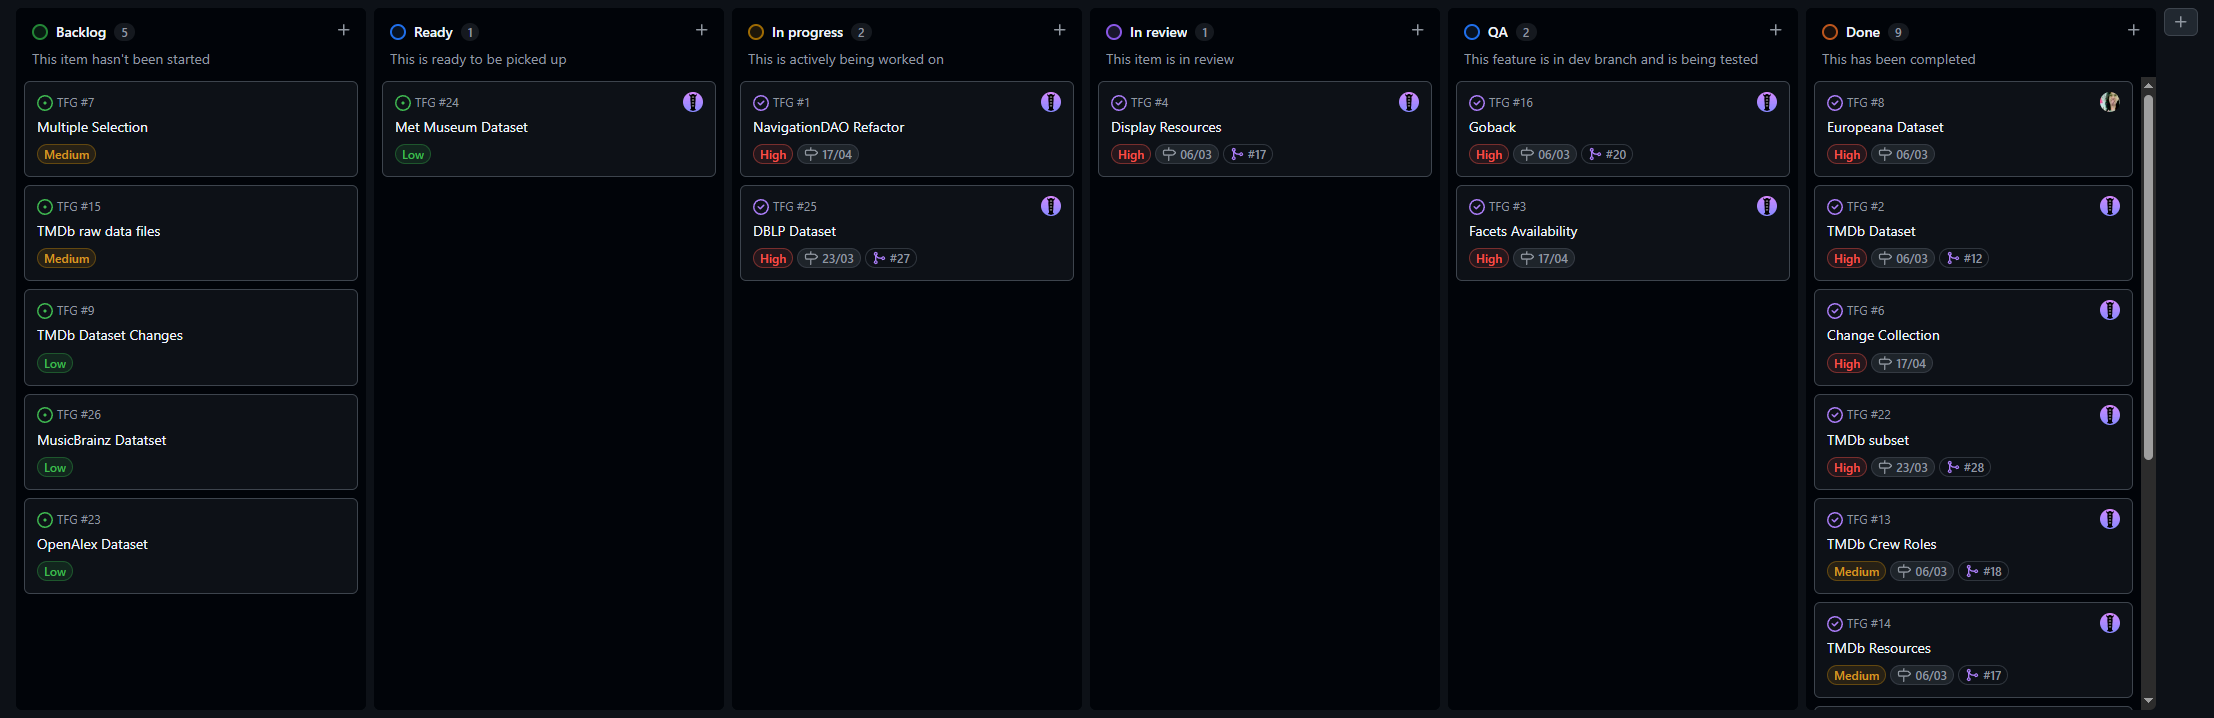
\includegraphics[width=1\textwidth]{Imagenes/Bitmap/backlog.png}
  \caption{Captura del backlog del proyecto en GitHub Projects.}
  \label{fig:backlog}
\end{figure}

    \subsection*{Trabajo colaborativo en un equipo reducido}

Hemos adaptado las práticas de \textbf{Scrum} a un entorno de colaboración directa y continua, ya que el proyecto sería 
desarrollado por un equipo de dos personas. En lugar de llevar a cabo reuniones formales, se optó por mantener una 
comunicación frecuente entre los integrantes, manteniendo siempre una divisón clara y acordada de responsabilidades, 
fundamental para la paralelización del desarrollo sin perder coherencia en el diseño global. Este método de comunicación 
y organización facilitó una evolución más eficiente y dinámica del software, con una alta capacidad de reacción 
frente los problemas técnicos.

    \subsection*{Control de versiones y gestión del código fuente}

En virtud de la necesidad de mantener la integridad del código y facilitar el trabajo colaborativo, hemos 
utilizado Git como sistema de control de versiones distribuido. El repositorio principal se alojó en GitHub\footnote{\url{https://github.com/hibjan/TFG}}
y se empleó una estrategia de ramificación sencilla : una rama principal (\texttt{main}) para el código 
estable y funcional, y ramas de características (\textit{feature branches}) para el desarrollo de nuevos 
componentes antes de su integración final. Con esa metodología, hemos podido trabajar en paralelo sin conflictos 
significativos manteniendo siempre una versión funcional del sistema.

    \subsection*{Buenas prácticas de programación y diseño}

Durante el desarrollo hemos dado especial atención a la aplicación de buenas prácticas de programación y 
diseño software. Se siguieron principios de separación de responsabilidades (\textit{Separation of Concerns}) 
y modularidad, lo cual está reflejado en la organización del código en distintos paquetes (por ejemplo, 
\texttt{controller}, \texttt{model}, \texttt{dao}, \texttt{filter}, etc.). Dicha estructura tiende a facilitar 
la legibilidad del código, su mantenimiento y la posibilidad de ampliación futura sin 
necesidad de realizar modificaciones significativas o profundas en su arquitectura.

\section{Arquitectura del Sistema}

Para permitir la exposición de la lógica del motor de exploración y su respectivo consumo por parte de aplicaciones, 
hemos diseñado una arquitectura fundamentada en el modelo Cliente-Servidor. Desde el lado del servidor (\textit{backend}), 
la aplicación favorece el desacoplamiento al basarse en capas bien definidas. Esta sección se dedica a detallar la capa de 
control, responsable de enrutar las distintas peticiones HTTP, y la capa de filtros, encargada de controlar las políticas 
de acceso y seguridad.

    \subsection*{Diseño de la API y Controladores}

Hemos optado por implementar la interfaz de comunicación entre el cliente web y el motor de navegación
usando una API de estilo REST, siguiendo la especificación de \textit{Servlets} de Java (\texttt{HttpServlet}) \citep{hunter2001servlets}.
Esta elección viene de priorizar un control directo sobre las peticiones y respuestas HTTP frente al uso de
frameworks web de más alto nivel (como Spring Boot), que aunque facilitan el desarrollo de aplicaciones web
tradicionales, introducen una mayor complejidad estructural y una capa adicional de abstracción que no resulta
necesaria para los objetivos de este proyecto.

El uso directo de \texttt{HttpServlet} ha sido necesaria para implementar una capa de comunicación más compacta, donde
cada controlador se encarga exclusivamente de recibir los parámetros de la petición, delegar la lógica en el
motor de navegación y generar la respuesta correspondiente en formato JSON. Emplear esa estrategia fue importante 
para mantener una separación explícita entre la lógica de navegación y la capa de acceso web. Además permitió un 
control más preciso de la gestión de sesiones, el formato de las respuestas y el flujo de las peticiones HTTP.

Para ejecutar la aplicación se ha utilizado Apache Tomcat \citep{brittain2007tomcat} como contenedor de \textit{Servlets}. Nos hemos inclinado por
Tomcat frente a otras opciones principalmente por la naturaleza del proyecto. Tomcat es un contenedor
considerablemente ligero, enfocado en la ejecución de aplicaciones basadas en \textit{Servlets} y JSP, lo que lo convierte en
una solución adecuada para trabajar directamente con la API de Java sin generar dependencias adicionales.

Por motivos semejantes, hemos descartado servidores de aplicaciones completos como GlassFish, 
ya que requieren tecnologías adicionales como EJB y gestión avanzada de recursos.
Alternativas como Jetty también permiten ejecutar \textit{Servlets}, pero éste está más orientado a una 
integración embebida dentro de otras aplicaciones/frameworks. Un contenedor independiente, 
sencillo de configurar y con respaldo de experiencia en entornos académicos y de desarrollo hace que 
Tomcat resulte la opción más estable encontrada.

Como contrapartida, esta decisión implica un mayor esfuerzo de implementación manual, especialmente en tareas
como el enrutamiento de peticiones, la serialización de datos o la gestión de errores. Sin embargo, este
\textit{trade-off} se ha asumido de forma consciente, ya que el objetivo principal del proyecto no es el
desarrollo de una aplicación web en sí, sino el diseño e implementación de un motor de navegación sobre
colecciones de datos, siendo la API web únicamente un mecanismo para exponer dicha funcionalidad.

    \subsection*{Gestión del Estado de Navegación (Enfoque \textit{Stateful})}

El manejo del contexto del usuario no es trivial, ya que, a diferencia de aplicaciones web tradicionales basadas 
en peticiones independientes, la naturaleza de nuestro proyecto implica una navegación que consiste en una exploración 
progresiva, donde cada acción del usuario modifica un estado acumulativo que condiciona las operaciones posteriores.

Las arquitecturas REST normalmente trabajan con sistemas \textit{stateless} (sin estado), donde cada petición del 
cliente debe contener toda la información necesaria para ser procesada. En nuestro caso, dicha naturaleza es altamente 
iterativa y acumulativa, de manera que hacer que cada petición esté completamente encapsulada y atomizada puede suponer 
un problema.

Requerir que el cliente envíe en cada petición el historial completo de navegación, las listas de filtros aplicados, 
las operaciones realizadas y los saltos relacionales supondría una sobrecarga de red inasumible. Este estado no puede 
considerarse independiente entre peticiones, sino que constituye una estructura dinámica que evoluciona a lo largo de 
la sesión de usuario. Además, requerir la petición completa añadiría una complejidad excesiva en el \textit{frontend}, 
aumentando el tamaño de cada \textit{request}, empeorando el rendimiento y dificultando considerablemente la escalabilidad.

Por este motivo, se ha optado por un diseño \textit{stateful}, en el que el contexto de navegación se mantiene en el 
servidor. Al inicio de la interacción, se crea una sesión de usuario (\texttt{HttpSession}) en la que se almacena una 
instancia de \texttt{StateManager}, encargada de gestionar el estado actual y las transiciones entre estados del usuario.

De este modo, los distintos controladores pueden operar sobre un contexto compartido y persistente, aplicando las 
acciones del usuario (como añadir filtros, explorar relaciones o combinar resultados) de forma centralizada en 
el \textit{backend}. Este enfoque permite simplificar la lógica del cliente, mejorar la eficiencia de las comunicaciones 
y mantener una coherencia estricta con el modelo de navegación propuesto.

    \subsection*{Componentes transversales de la arquitectura}

El sistente contiene una serie de componentes transversales, más allá de la capa de controladores, que proporcionan 
funcionalidades comunes que permiten separar claramente la lógica de dominio y los aspectos técnicos propios de la 
infraestructura web.

Como se ha mencionado en la sección anterior, la gestión de sesiones es un elemento fundamental dentro de la arquitectura, pues 
es el responsable por mantener el contexto de navegación del usuario entre peticiones distintas. A través del mecanismo de
\texttt{HttpSession}, el sistema asocia cada usuario con una instancia de \texttt{StateManager}, lo que 
garantiza la persistencia del estado de navegación y posibilita un modelo de interacción basado en estados.

Por otro lado, la serialización de datos en formato JSON empleada de manera sistemática funciona como el mecanismo 
clave para el intercambio de información entre el \textit{backend} y el \textit{frontend}. Este abordaje se ha hecho necesario principalmente 
para desacoplar ambas capas, lo que facilita la evolución independiente de la interfaz de usuario y del motor de navegación
como tal.

Adicionalmente, hemos implementado un filtro encargado de gestionar aspectos técnicos de la comunicación HTTP,
como el intercambio de recursos entre distintos orígenes - política CORS \textit{(Cross-Origin Resource Sharing)}. 
Este componente intercepta las peticiones entrantes antes de que alcancen los controladores y añade 
las cabeceras necesarias para permitir la comunicación entre cliente y servidor cuando se ejecutan en 
dominios o puertos distintos, necesario para evitar las restricciones por defecto de seguridad del navegador. De este modo, 
se evita introducir lógica técnica adicional en los controladores y se mantiene su enfoque en la lógica de dominio.

\section{Persistencia y Acceso a Datos}

La capa de persistencia y su respectivo diseño constituyen la base fundamental de la arquitectura del sistema, 
puesto que el motor de navegación tiene una relación de depencia directa de la estructura y disponibilidad de los 
datos sobre los que opera. Como el sistema no se limita a recuperación de la información, en este proyecto los datos no 
se consumen directamente, sino que pasan por una transformación y reorganización que permiten la exploración mediante 
un modelo de navegación relacional.

Para posibilitar dicha exploración y mantener un nivel razonable de independencia del dominio, hemos decidido desacoplar 
completamente la lógica del motor de las fuentes de datos concretas. Para ello, hemos definido un modelo interno de representación 
que abstrae las entidades y relaciones relevantes del dominio, permitiendo trabajar de forma uniforme independientemente del origen de los
datos. Este enfoque es particularmente relevante dado que el sistema integra conjuntos de datos heterogéneos, los cuales deben ser 
"traducidos" \ bajo una misma estructura conceptual.

Por ese misma razón, hemos optado por organizar el acceso a datos a través de una capa dedicada de abstracción \textit{(DAO)}, 
que se encarga de aislar la lógica de acceso, traducción y recuperación de la información. Esta separación es lo que garantiza mantener 
la independencia entre la lógica de navegación y los mecanismos de persistencia, permitiendo al mismo tiempo una evolución del proprio sistema 
y posible cambios en las fuentes de datos o incluso en su forma de almacenamiento.

    \subsection*{Modelo de datos y representación interna}

El sistema se base en un modelo de datos interno diseñado específicamente para soportar la navegación
sobre colecciones complejas, permitiendo representar relaciones cualitativamente distintas independiente del dominio asociado.  
Decidimos no operar directamente sobre las estructuras proporcionadas por las fuentes de datos externas, y sí definir una representación 
propia basada en entidades y relaciones, adaptada a las necesidades del motor de navegación.

En dicho modelo, los elementos del dominio se representan como entidades independientes, caracterizadas
por un conjunto de atributos (\textbf{metadatos}), mientras que las interacciones entre dichas entidades se
expresan mediante relaciones explícitamente manifiestas. Esta separación permite tratar de forma homogénea tanto el
filtrado por atributos (por ejemplo, características propias de una entidad) como la exploración
relacional (navegación entre entidades conectadas).

Al mismo tiempo, esta representación actúa como una capa de abstracción sobre las fuentes de
datos, unificando conjuntos heterogéneos bajo una estructura común e independiente de su formato u origen.
De este modo, el motor de navegación puede operar de forma desacoplada, garantizando tanto la extensibilidad
del sistema como la coherencia en las operaciones realizadas sobre los datos.

    \subsection*{Integración y adquisición de datos}

Dado que el sistema utiliza y transforma fuentes de datos heterogéneas, una de las decisiones
arquitectónicas principales ha sido definir un proceso de integración que permita desacoplar la
adquisición de datos de su representación interna. En lugar de depender directamente de la estructura
y organización de cada fuente, se ha establecido un mecanismo de transformación que adapta los datos
externos al modelo común basado en entidades y relaciones descrito anteriormente.

Este proceso de integración implica la extracción de la información relevante de cada fuente de datos,
su normalización y su posterior adaptación a las estructuras internas del sistema. De este modo, se
garantiza que, independientemente del formato, granularidad o semántica original de los datos, todos
ellos puedan ser tratados de forma uniforme por el motor de navegación.

Una de las consideraciones más importantes en este diseño ha sido la coexistencia de distintos conjuntos de datos
con características complementarias. Antes de privilegiar una única fuente como referencia principal,
hemos diseñado el sistema para permitir la incorporación de nuevas fuentes, siempre que estas
puedan ser mapeadas al modelo interno. Este enfoque posibilita la extensibilidad del sistema y evita
dependencias estríctas con tecnologías o fuentes concretas.

Asimismo, se ha optado por un modelo de integración en el que la responsabilidad de adaptación recae en
la capa de acceso a datos, evitando trasladar esta complejidad al motor de navegación. De este modo, el
núcleo del sistema opera exclusivamente sobre estructuras homogéneas, manteniendo una separación clara
entre la lógica de dominio y los detalles específicos de cada fuente de datos.

    \subsection*{Capa de acceso a datos (DAO)}

Para mantener una separación eficiente entre la lógica de navegación y los mecanismos de acceso
a datos, hemos definido una capa específica de abstracción basada en el patrón \textit{Data Access Object} (DAO).
La capa actúa como intermediaria entre el modelo interno del sistema y las distintas fuentes de datos,
encapsulando toda la lógica necesaria para la recuperación y adaptación de la información.

La principal responsabilidad de los componentes DAO es proporcionar una interfaz uniforme de acceso a los datos,
independiente de su origen. De este modo, el motor de navegación no interactúa de manera directa con las fuentes externas,
sino que opera sobre estructuras ya adaptadas al modelo interno. Hemos tomado esta decisión para aislar completamente el núcleo
del sistema de detalles específicos (como el formato de los datos, los mecanismos de acceso o, mismamente, las 
particularidades de cada fuente).

Además, esta capa facilita la integración de múltiples conjuntos de datos, ya que cada fuente puede ser gestionada
mediante su propia implementación de acceso, de manera compleamente independiente, sin afectar al resto del sistema. 
Esto resulta especialmente relevante en un contexto donde hay una coexistencia de datos heterogéneos, permitiendo 
su incorporación de manera progresiva, controlada y sin grandes dependencias.

Esta decisión también es relevante para hacer la mantenibilidad y evolución del sistema de manera flexible. Al centralizar
la lógica de acceso a datos en una capa específica, es posible realizar cambios en las fuentes de información,
en sus formatos o en las estrategias de recuperación sin necesidad de modificar el motor de navegación o la
capa de control. Por lo tanto, se garantiza una arquitectura modular, robusta, preparada para futuras extensiones y 
la incorporación de otras colecciones de datos.

    \subsection*{Estrategias de gestión de datos}

Como mencionado anteriormente, hemos priorizado el diseño del sistema a partir de una separación clara entre dos niveles de 
gestión de datos: el estado de navegación del usuario y los datos del dominio. Esta distinción responde a criterios
distintos de persistencia, mutabilidad y coste de acceso, y determina la arquitectura general del sistema.

Los datos del dominio --- entidades, metadatos y relaciones --- se almacenan de forma persistente
en una base de datos relacional. Esta decisión facilita que el sistema soporte datasets de tamaño
potencialmente grandes sin imponer restricciones sobre la memoria disponible, y delega en el motor de base
de datos la responsabilidad de ejecutar las operaciones de filtrado y recuperación de forma
razonable.

El estado de navegación, en cambio, es ligero, momentáneo y específico de cada usuario: recoge los
filtros acumulados, el historial de transiciones entre colecciones y los conjuntos de resultados
en construcción. Hemos decidido mantenerlo en memoria dentro de la sesión HTTP por su naturalidad, 
dado su ciclo de vida acotado y su reducido tamaño, además de evitar serializar y deserializar el contexto de 
navegación en cada petición.

La consecuencia más relevante de esta separación es que el sistema no materializa subconjuntos
intermedios de resultados: en cada petición, el estado en memoria se traduce directamente a una
consulta sobre la base de datos. Esto simplifica el modelo de datos a costa de trasladar la
complejidad al proceso de construcción dinámica de queries, que debe reflejar fielmente el
contexto de navegación acumulado. Esta tensión --- entre simplicidad del modelo y complejidad de
las consultas --- es una de las decisiones de diseño que hemos estimado que tendría un gran impacto en la implementación,
y se aborda en detalle en el capítulo siguiente.